% !TEX root = ~/OpenFOAM/antoniopucciarelli-9/run/LABS/thermochemical_CFD/main.tex

\section{Compressible flow - $\mathtt{Lab04}$}
    
    \renewcommand{\thepage}{\arabic{page}}
    \setcounter{page}{\thelastPage}
In~\ref{app:app2} are described the main equations, concepts and possible OpenFOAM implementation for compressible flows.

%    \subsection{Energy equation}
%With respect to the incompressible case, the compressible case enables the changes in $\rho$ of the fluid. This new degree of freedom in the system has to be treated with care using the energy equation. The energy equation has different forms that suit best for defined physical behaviours in the system\footnote{$h$ is the specific enthalpy, $e$ is the specific internal energy, $K$ is the total kinetic energy and $E$ is the total energy.}:

%{\small
%\begin{align} 
%    \frac{\partial \rho e}{\partial t} + \boldsymbol{\nabla} \cdot \big( \rho \boldsymbol{u} e \big) + \frac{\partial \rho K}{\partial t} + \boldsymbol{\nabla} \cdot \big( \rho \boldsymbol{u} K \big) + \boldsymbol{\nabla} \cdot \big( \boldsymbol{u} p \big) = - \boldsymbol{\nabla} \cdot \boldsymbol{q} + \boldsymbol{\nabla} \cdot \big( \boldsymbol{\tau} \cdot \boldsymbol{u} \big) + \rho r + \rho \boldsymbol{g} \cdot \boldsymbol{u} \label{eqn:heqn} \\  
%    \frac{\partial \rho h}{\partial t} + \boldsymbol{\nabla} \cdot \big( \rho \boldsymbol{u} h \big) + \frac{\partial \rho K}{\partial t} + \boldsymbol{\nabla} \cdot \big( \rho \boldsymbol{u} K \big) - \frac{\partial p}{\partial t} = - \boldsymbol{\nabla} \cdot \boldsymbol{q} + \boldsymbol{\nabla} \cdot \big( \boldsymbol{\tau} \cdot \boldsymbol{u} \big) + \rho r + \rho \boldsymbol{g} \cdot \boldsymbol{u} \label{eqn:eeqn} \\  
%    \frac{\partial \rho E}{\partial t} + \boldsymbol{\nabla} \cdot \big( \rho \boldsymbol{u} E \big) + \boldsymbol{\nabla} \cdot \big( \boldsymbol{u} p \big) = - \boldsymbol{\nabla} \cdot \boldsymbol{q} + \boldsymbol{\nabla} \cdot \big( \boldsymbol{\tau} \cdot \boldsymbol{u} \big) + \rho r + \rho \boldsymbol{g} \cdot \boldsymbol{u} \label{eqn:Eeqn}  
%\end{align}. 
%}

%One of the most used energy equation is in the $h$ formulation~\cite[Ch. 11]{ferziger2002computational}. The $h$ formulation uses $h = e + \frac{p}{\rho}$ and $K$ as \textit{thermodynamic} and \textit{mechanical} energy describers. In both $h - e$ formulations, $K$ is always computed; instead in the total energy formulation, $K$ is hidden in $E = e + K$. Most of the energy formulations in OpenFOAM neglect the mechanical part $\boldsymbol{\nabla} \cdot \big( \boldsymbol{\tau} \cdot \boldsymbol{u} \big)$ and $\rho \boldsymbol{g} \cdot \boldsymbol{u}$.  

%In the whole assignment, the compressibility is treated with the $h$ formulation. The reason about this choice relies on the physics of the problem: for a problem with heat flux and with combustion of a non premixed mixture, the $h$ formulation is preferred.

%\subsubsection{$h$ equation in OpenFOAM}
%There are different ways for solving the compressible flow problems. The philosophy stays the same. One of the possible $h$ formulations is described in \verb|rhoPimpleFoam| and the main codes used in it are \verb|pEqn.H|, \verb|UEqn.H|, \verb|EEqn.H| and \verb|rhoPimpleFoam.C|. 

%The main parts of \verb|rhoPimpleFoam.C| are the following: 
%\begin{itemize}
%    \item \textbf{Outer loop}
%    \begin{itemize}
%        \item \textbf{$\rho$ computation} - \verb|rhoEqn.H| - Since $\rho$ is a derived field, it needs to be computed. 
%        \item \textbf{$\boldsymbol{u}$ predictor} - \verb|UEqn.H| - Computation of a first $\boldsymbol{u}$ approximation. 
%        \item \textbf{$h$ equation} - \verb|EEqn.H|\cprotect\footnote{\verb|EEqn.H| uses \verb|dpdt|. \verb|dpdt| is computed in \verb|pEqn.H| with \verb|dpdt = fvc::ddt(p)|.} - Computation of the $h - T$ field through guessed $\rho - p^*$ and the previous predicted $\boldsymbol{u}$. 
%        \item \textbf{Inner loop}
%        \begin{itemize}
%            \item \textbf{$p$ corrector} - \verb|pEqn.H|\cprotect\footnote{The Helmoltz equation can be seen as a Poisson equation with a $\frac{\partial \rho}{\partial t}$ term that is converted in $p$ terms and then treated implicitly.} - Guarantee continuity with Helmolts equation.
%            \begin{itemize}
%                \item \textbf{$\frac{\partial p}{\partial t}$ computation} Computation of $\frac{\partial p}{\partial t}$ needed in $h$ formulation.
%            \end{itemize}
%            \item \textbf{$\rho$ computation/correction} - \verb|rhoEqn.H| - Correcting again $\rho$ field with new $p$ field and the $T$ field from the $h$ equation solution.
%    \end{itemize}
%    \end{itemize}
%    \item \textbf{Convergence check}
%    \item \textbf{Time step advancement}
%    \begin{itemize}
%        \item \textbf{Guessed fields for the new time step} The new time step gets the guessed values from the last time step solutions.
%    \end{itemize}
%\end{itemize}

%\subsubsection{$\psi$ and $\rho$ based model}
%In CFD there are many ways for coupling the energy, pressure, velocity equations and the equation of state. All these ways for the computation of $\rho$ can be separated in 2 families: the pressure based $\psi$ equation and the $\rho$ based equations. 

%\paragraph{$\psi$} The $\psi$ based equations uses an explicit relation between $\rho$ and $p$ through $\psi$. An example is the $\psi$ equation that is based on the equation of the perfect gases, $\psi = \frac{1}{R T}$ such that $\rho = \psi \cdot p$. This family of models are best suitable for the segregated (semi-implicit) method because it is a \textbf{$p$ based} algorithm.

%\paragraph{$\rho$} The $\rho$ based equations are another set of equations that allow the computation of $\rho$ through a $\rho$ dependent PDE or through an equation that does not explicitly relate $\rho$ to $p$ such as the \textbf{Boussinesque approximation} $\Delta \rho = \beta \Delta T$.

\subsection{Problem setup}
\subsubsection{Boundary conditions}
The main changes in the boundary conditions in \verb|0/| folder are:
\subparagraph{$p$} Due to the presence of pressure waves, because the hyperbolic formulation of the problem, the outlet boundary condition has to be changed. As result of this, the outlet allows pressure waves to pass through and it allows also to not over-constraint the problem. So the outlet is set as \verb|waveTransmissive| type and with the pressure field at infinite equal to \verb|internalField|. Of course, the dimension of $p$ has to change because now the problem is no more formulated as $\frac{p}{\rho}$. 
\subparagraph{$\alpha_t$} Due to the compressibility, the problem has to deal with turbulent heat transfer coefficient $\alpha_t$. All the $\alpha_t$ are set as \verb|calculated| except at the walls where it is used a wall function \verb|compressible::alphatWallFunction|\footnote{The use of wall functions in $\kappa$, $\varepsilon$, $\nu_t$ and $\alpha_t$ is related to the fact that the centres of all the nearest control volumes to the walls are at $y^+ > 10$ and so out of the \textbf{viscous subregion}. Being out of this region it is necessary compute with the wall function these values. This will result in exploiting the results of theory: \textbf{log-law} model adoption.}.   
\subparagraph{$T$} Setting $T$ boundary conditions is like setting $h$ boundary conditions, because their relation. The \verb|T| file changes for each problem because different boundary conditions at the walls and the flow field temperature.

\subsubsection{Schemes}
\cprotect\paragraph{\verb|fvSchemes|}
New schemes are added such \verb|div(phi,h)| and \verb|div(phi,K)| that allow to compute $\boldsymbol{\nabla} \cdot \big( \rho \ \boldsymbol{u} \ h \big)$ and $\boldsymbol{\nabla} \cdot \big( \rho \ \boldsymbol{u} \ K \big)$ respectilvely.

\verb|wallDist| is a new function that describes the method used for the \verb|waveTransmissive| type in \verb|p|.

\cprotect\paragraph{\verb|fvSolution|}
The compressible case has to deal also with how to solve the energy equations, so solution schemes and tolerances are declared as well as $p$ and $U$ for $h$.

\cprotect\subsubsection{\verb|thermophysicalProperties|}
This file allows to describe the way the equation of energy is solved and how to compute $\rho$ from the available fields. 
\cprotect\paragraph{\verb|thermoType|}
This part of the dictionary declares how to solve energy and $\rho$ through \verb|hePsiThermo|.
\begin{itemize}
    \item \verb|hePsiThermo| - \verb|type| - allows the usage of the equation of energy base on $h - e$ and the usage of $\psi$ based method for the computation of $\rho$ (so explicitly related to $p$). 
    \item \verb|pureMixture| - \verb|mixture| - allows treating a single mixture in gaseous phase.
    \item \verb|perfectGas| - \verb|equationOfState| - allows using the perfect gas equation $\rho~=~\frac{p}{R T}$ for $\psi$.
    \item \verb|sensibleEnthalpy| - \verb|energy| - allows using the $h$ formulation for the energy equation.
\end{itemize}

\cprotect\paragraph{\verb|mixture|}
This part of the dictionary declares the mixture properties. 

The following \verb|mixture| properties are related to gas propeties:
\begin{itemize}
    \item \verb|specie| sets the molecular weight of the substance - air in this case -.
    \item \verb|thermodynamics| sets the thermodynamics relations between $T$ and $h$; based on constants as expressed in \verb|thermoType -> thermo hConst;|
    \item \verb|transport| sets transport properties of the mixture and are set to \verb|const| in \verb|thermoType -> transport const;|.
\end{itemize}

\verb|dpdt yes;| enables the usage of $\frac{\partial p}{\partial t}$ used in the $h$ formulation. 

\subsection{Post-processing}
All the post-processing functions, except the residual function, print the field with time interval $\Delta t = 0.1 s$ in order to save disk space. 
\cprotect\subsubsection{\verb|MachNo|}
This is a post-process function that enables the computation of Mach field using $Ma = \frac{U}{\sqrt{\gamma R T }}$. 

\subsection{Results}    
\cprotect\subsubsection{\verb|combustorRhoPimple_lowT_lowRe|}
This simulation was set \verb|maxCo 5.0;|. Vortex shedding is present in the field. With respect to the other fields, pressure waves travel at lower speed, this brings to a longer time for the velocity to change.   

\cprotect\subsubsection{\verb|combustorRhoPimple_highT_lowRe|}
This simulation starts to show instability effects from the last few steps of the simulation. The pressure wave speed\footnote{$c = \sqrt{\gamma \ R \ T}$.} is higher than in the \verb|combustorRhoPimple_lowT_lowRe| case.

\cprotect\subsubsection{\verb|combustorRhoPimple_hightT_highRe|}
As the previous simulation, flow instability effects start to be present in the final solution steps. 

\newpage

% PAGE MANAGEMENT
% saving page number
\setcounter{lastPage}{\thepage}
% changing page numbering for the results figures
\setcounter{page}{1}
\renewcommand{\thepage}{COM-\roman{page}}

\begin{figure}[!h]
    \centering
    \import{latexFIGS/lab04/}{residuals.pgf}
    \caption{Compressible cases: residuals.}
    \label{fig:residualComp}
\end{figure}

\begin{figure}[!h]
    \centering
    \import{latexFIGS/lab04/}{T.pgf}
    \caption{Compressible cases: $T$ profile at $y = 100mm$.}
    \label{fig:Tcomp}
\end{figure}

\begin{figure}[!h]
    \centering
    \import{latexFIGS/lab04/}{Uy.pgf}
    \caption{Compressible cases: $U_y$ profile at $y = 100mm$.}
    \label{fig:UyCOMP}
\end{figure}

\begin{figure}[!h]
    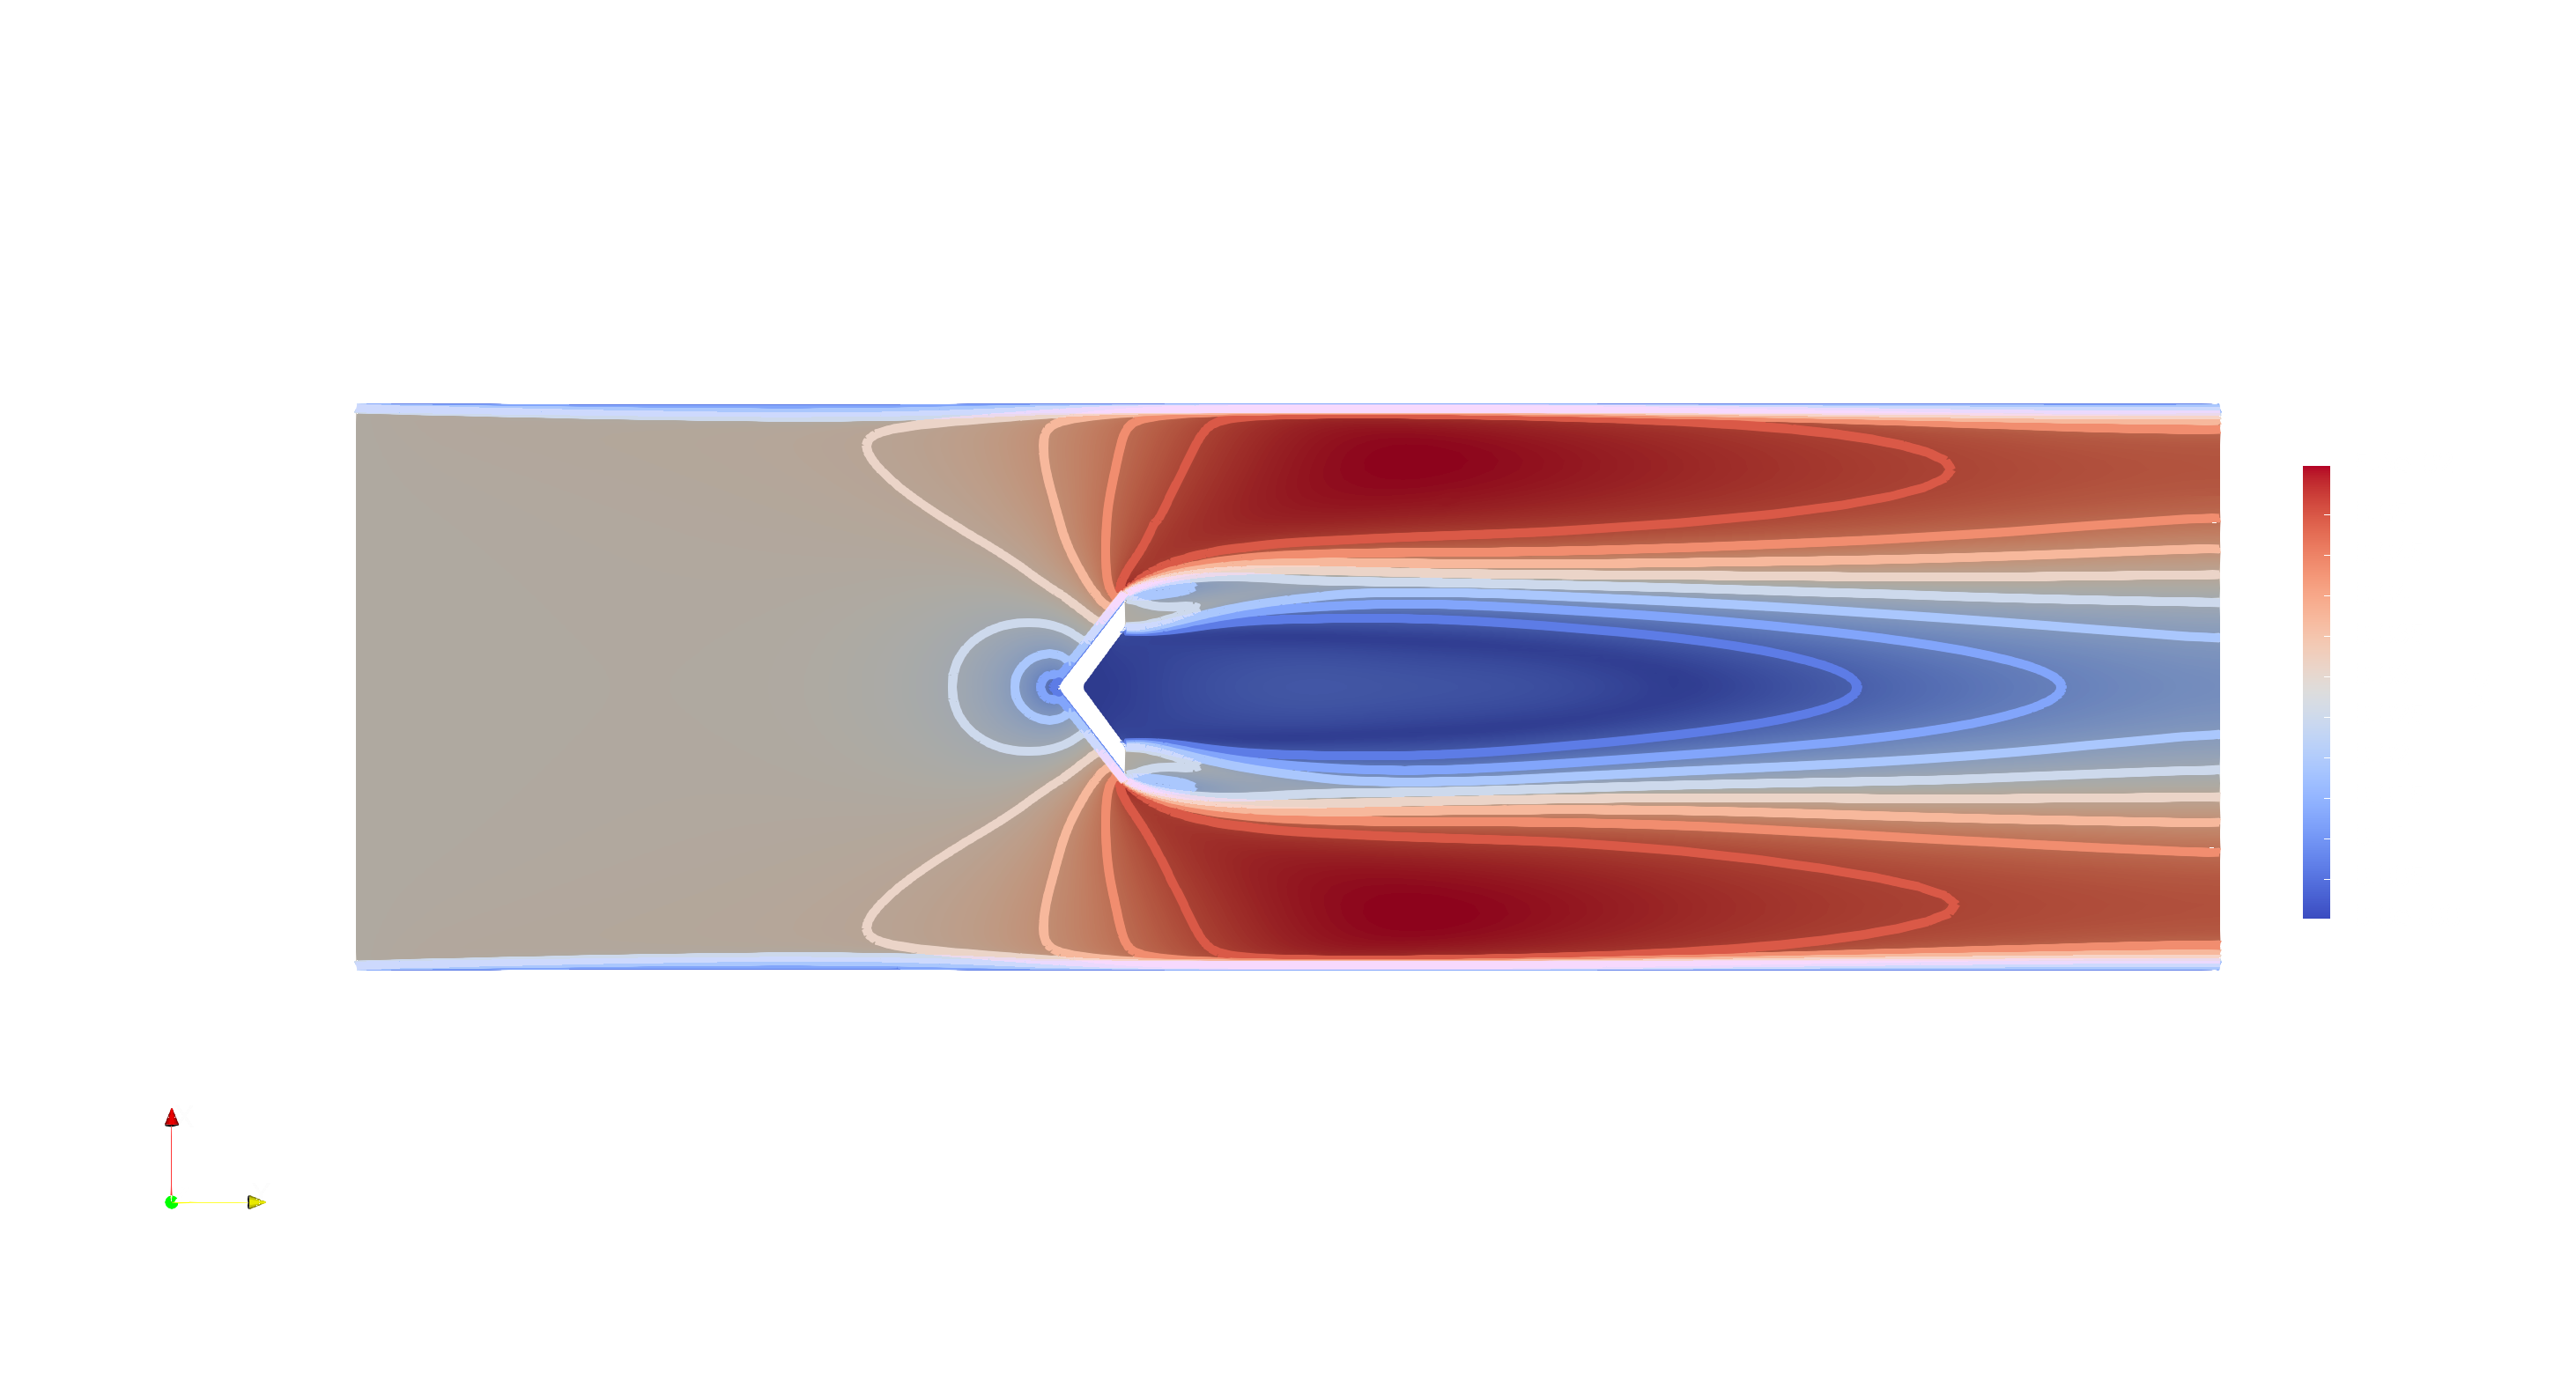
\includegraphics[width=\textwidth]{latexFIGS/figs/combustorMachHL.png}
    \cprotect\caption{Mach isolines for \verb|combustorRhoPimple_highT_lowRe| at $t = 0.4s$.}
\end{figure}

\begin{figure}[!h]
    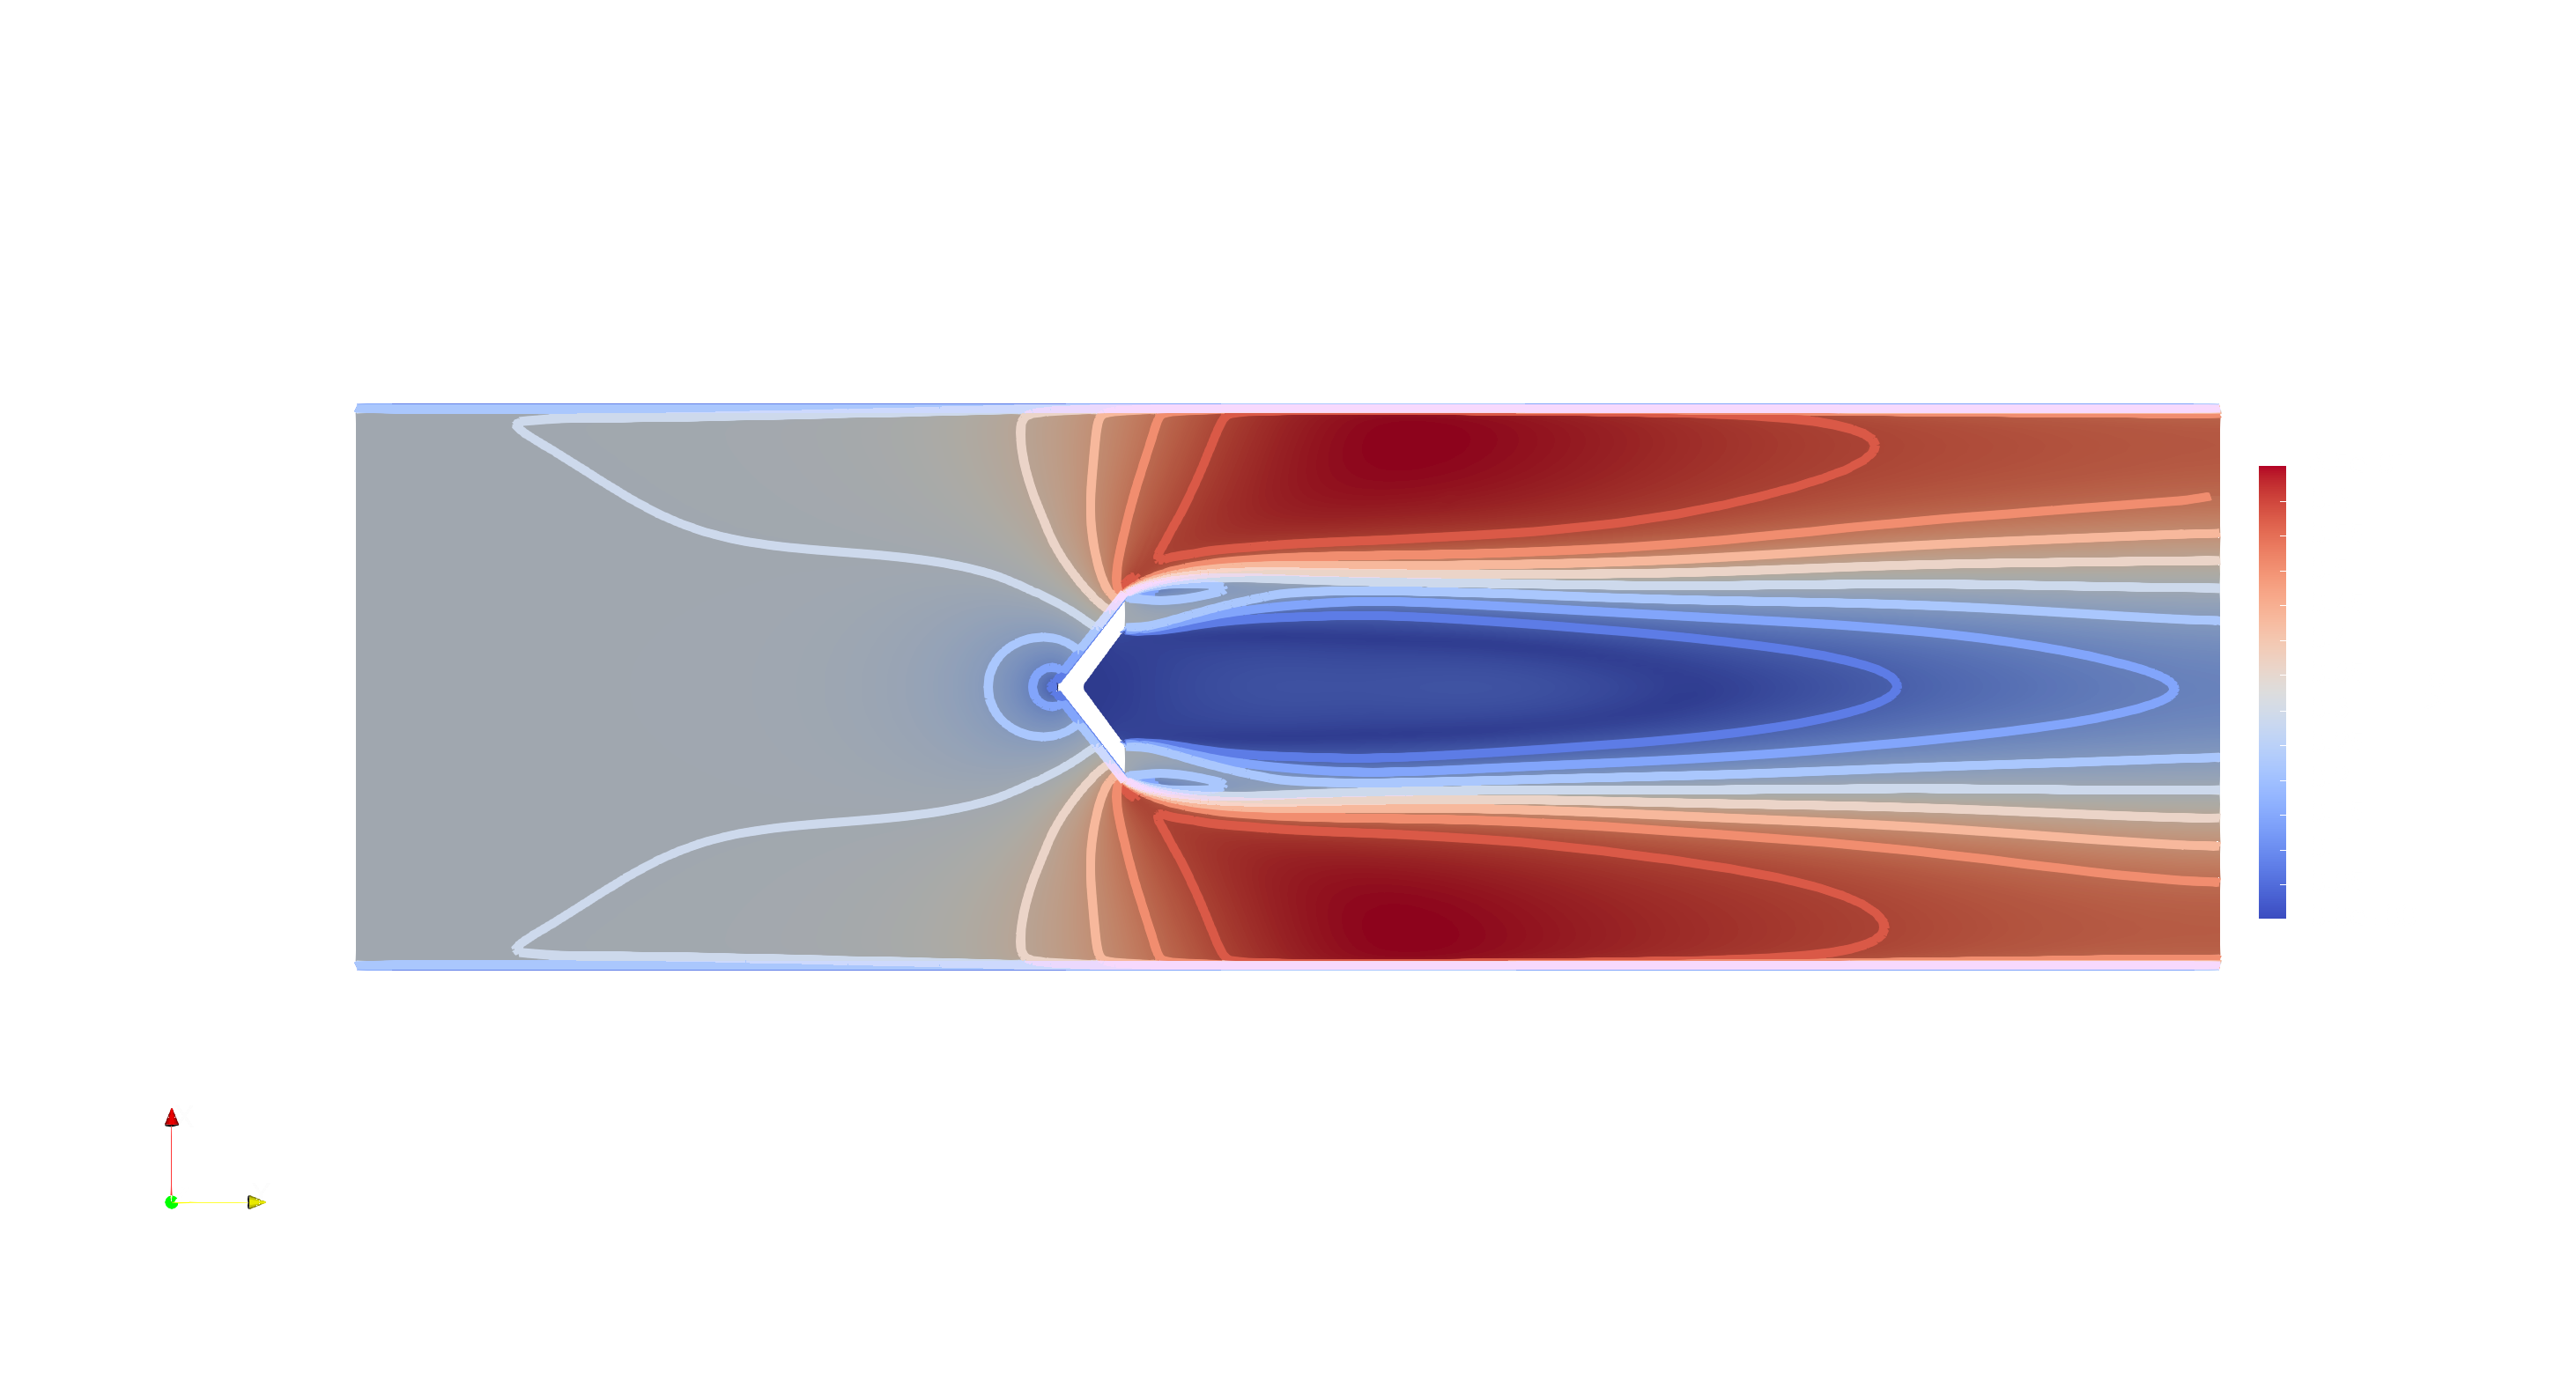
\includegraphics[width=\textwidth]{latexFIGS/figs/combustorMachHH.png}
    \cprotect\caption{Mach isolines for \verb|combustorRhoPimple_highT_highRe| at $t = 0.4s$.}
\end{figure}

\clearpage
